% Gemini theme
% https://github.com/anishathalye/gemini

\documentclass[final, 20pt]{beamer}

% ====================
% Packages
% ====================

\usepackage[T1]{fontenc}
\usepackage{lmodern}
\usepackage[size=custom,height=91.44, width=121.92,scale=1.0]{beamerposter}
\usetheme{gemini}
\usecolortheme{mit}
\usepackage{graphicx}
\usepackage{booktabs}
\usepackage{tikz}
\usepackage{pgfplots}

\usepackage[pinyin, english]{babel}
%\usepackage[utf8]{inputenc}

\usepackage{amsmath}
\usepackage{amsfonts}
\usepackage{amsthm}
\usepackage{bm}
\usepackage{xcolor}
\usepackage{multirow}
\usepackage[normalem]{ulem}
\usepackage{pifont}
\usepackage{array}
\usepackage{multimedia}
\usepackage{makecell}
\usepackage{xspace}
\usepackage{luatexja-fontspec}

\graphicspath{{../slides/figures/}}

\DeclareMathOperator*{\argmin}{\arg\!\min}
\DeclareMathOperator*{\argmax}{\arg\!\max}
\DeclareMathOperator*{\substr}{substr}
\DeclareMathOperator*{\subseq}{subseq}
\DeclareMathOperator*{\len}{len}

\newcommand\BibTeX{B{\sc ib}\TeX}
\newcommand{\abr}[1]{\uppercase{#1}}
\newcommand{\nlp}{\textsc{nlp}}
\newcommand{\mb}[1]{\boldsymbol{\mathbf{#1}}}
\newcommand{\g}{\, | \,}
\newcommand{\mtanchor}{MTAnchor\xspace}
\newcommand{\ch}[2]{#1 (#2)}
\setmainjfont{FandolSong}

\newcommand{\header}[1]{\begin{center}\heading{#1}\end{center}}

% ====================
% Lengths
% ====================

% If you have N columns, choose \sepwidth and \colwidth such that
% (N-1)*\sepwidth + N*\colwidth + 2*\edgewidth = \paperwidth
\newlength{\sepwidth}
\newlength{\colwidth}
\newlength{\edgewidth}
\setlength{\sepwidth}{0.01\paperwidth}
\setlength{\colwidth}{0.22\paperwidth}
\setlength{\edgewidth}{0.045\paperwidth}

\newcommand{\separatorcolumn}{\begin{column}{\sepwidth}\end{column}}

\newcommand{\edgecolumn}{\begin{column}{\edgewidth}\end{column}}

% ====================
% Title
% ====================

\title{Multilingual Anchoring: Interactive Topic Modeling and Alignment Across Languages}

\author{Michelle Yuan \inst{1} \and Benjamin Van Durme \inst{2} \and Jordan Boyd-Graber \inst{1}}

\institute[shortinst]{\inst{1} University of Maryland \samelineand \inst{2} John Hopkins University}

% ====================
% Body
% ====================

\begin{document}

\begin{frame}[t]
\begin{columns}[t]
\edgecolumn

\begin{column}{\colwidth}


\begin{block}{Motivation}
	\begin{itemize}
		\item Large text collections often require topic triage quickly in low-resource settings (e.g. natural disaster, political instability)
		\item Analysts need to examine multilingual documents but are scarce in one or more languages
	\end{itemize}
\end{block}


  \begin{block}{Modeling Multilingual Topics}
	
%	Given documents of different languages, we want to extract common topics from them.  In a multilingual topic model, topics are distributions over words in different languages. 
	
	\begin{figure}
	\centering
	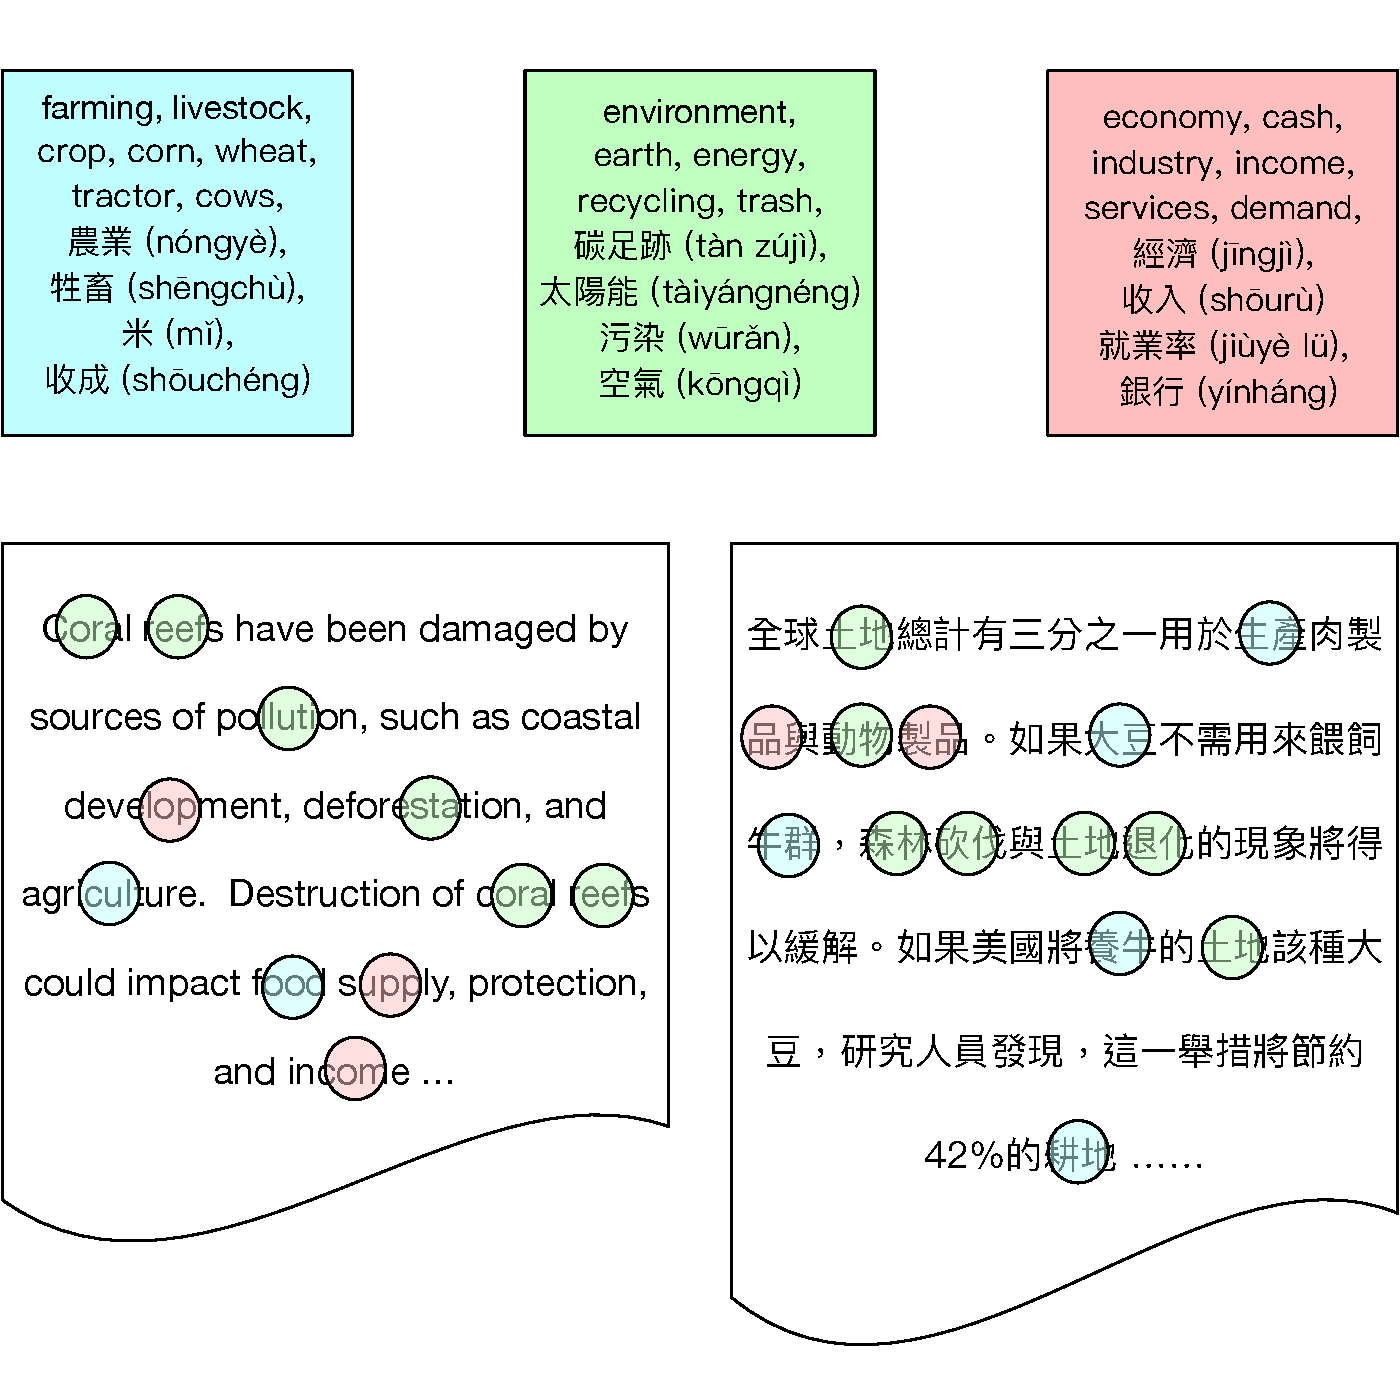
\includegraphics[width=0.7\linewidth]{articles5}
	\end{figure}




  \end{block}

  \begin{block}{Anchor-based Topic Models}

\begin{itemize}
    \item  An \textbf{anchor word} is a word that appears with high probability in one topic and low probability in all other topics
    \item Conditional co-occurrence matrix $\bar{Q}$ has entries such that \(\bar{Q}_{i,j} = p(\text{word 2} = j \g \text{word 1} = i) \)
    \item Given anchor words \(s_1, \dots,s_K\), the algorithm approximates \(\bar{Q}_{i}\) as the convex combination of \(\bar{Q}_{s_1}, \dots \bar{Q}_{s_K} \) and finds coefficients $C_{i,k}$ that estimate $p(\text{topic} = k \g \text{word}=i )$
\end{itemize}
   
    	
%	\begin{figure}
%	\centering
%	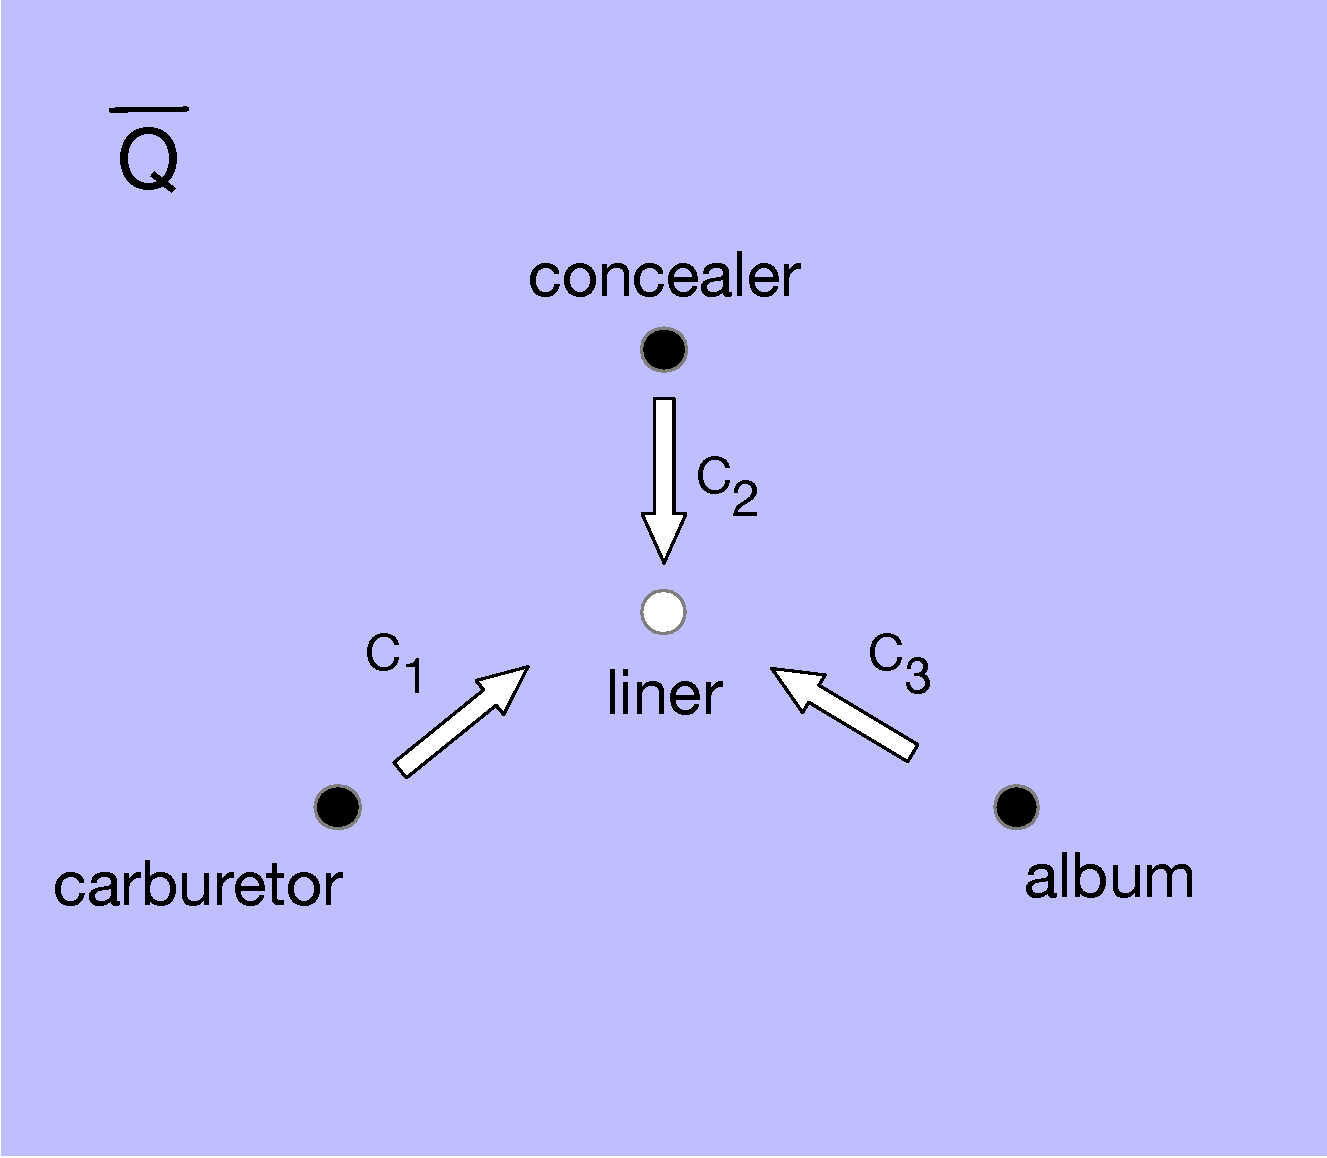
\includegraphics[width=0.6\linewidth]{combination}
%	\end{figure}

\begin{table}[]
	\begin{tabular}{lllll}
		\textbf{$\bar{Q}$ matrix} & carburetor                & concealer                 & album                     & liner                     \\ \cline{2-5} 
		\multicolumn{1}{l|}{carburetor} & \multicolumn{1}{l|}{0.80} & \multicolumn{1}{l|}{0.05} & \multicolumn{1}{l|}{0.05} & \multicolumn{1}{l|}{0.10} \\ \cline{2-5} 
		\multicolumn{1}{l|}{concealer}  & \multicolumn{1}{l|}{0.13} & \multicolumn{1}{l|}{0.60} & \multicolumn{1}{l|}{0.07} & \multicolumn{1}{l|}{0.20} \\ \cline{2-5} 
		\multicolumn{1}{l|}{album}      & \multicolumn{1}{l|}{0.05} & \multicolumn{1}{l|}{0.05} & \multicolumn{1}{l|}{0.70} & \multicolumn{1}{l|}{0.20} \\ \cline{2-5} 
		\multicolumn{1}{l|}{liner}      & \multicolumn{1}{l|}{0.25} & \multicolumn{1}{l|}{0.20} & \multicolumn{1}{l|}{0.15} & \multicolumn{1}{l|}{0.45} \\ \cline{2-5} 
	\end{tabular}
\end{table}

\begin{equation}
\bar{Q}_{\text{liner}} \approx C_1 \bar{Q}_{\text{carburetor}} + C_2 \bar{Q}_{\text{concealer}} + C_3 \bar{Q}_{\text{album}}
\label{eq:q}
\end{equation}


This decomposition (Eq.~\ref{eq:q}) resembles the topic distribution of ``liner'' over an \underline{automotive} topic, a \underline{cosmetics} topic, and a \underline{music} topic.
 
\end{block}

\end{column}

\separatorcolumn


\begin{column}{1.25\colwidth}

  \begin{block}{Bridging Languages: How Do You Say Anchor in Chinese?}
  	
  	\begin{columns}[t, totalwidth=\linewidth]
	
	\begin{column}{0.27\textwidth}
	\header{Monolingual Anchoring}
	
    
    Rows in $\bar{Q}$ corresponding to the anchor words are the vertices of the convex hull formed by $\bar{Q}$. 
    
    \begin{figure}
    	\centering
    	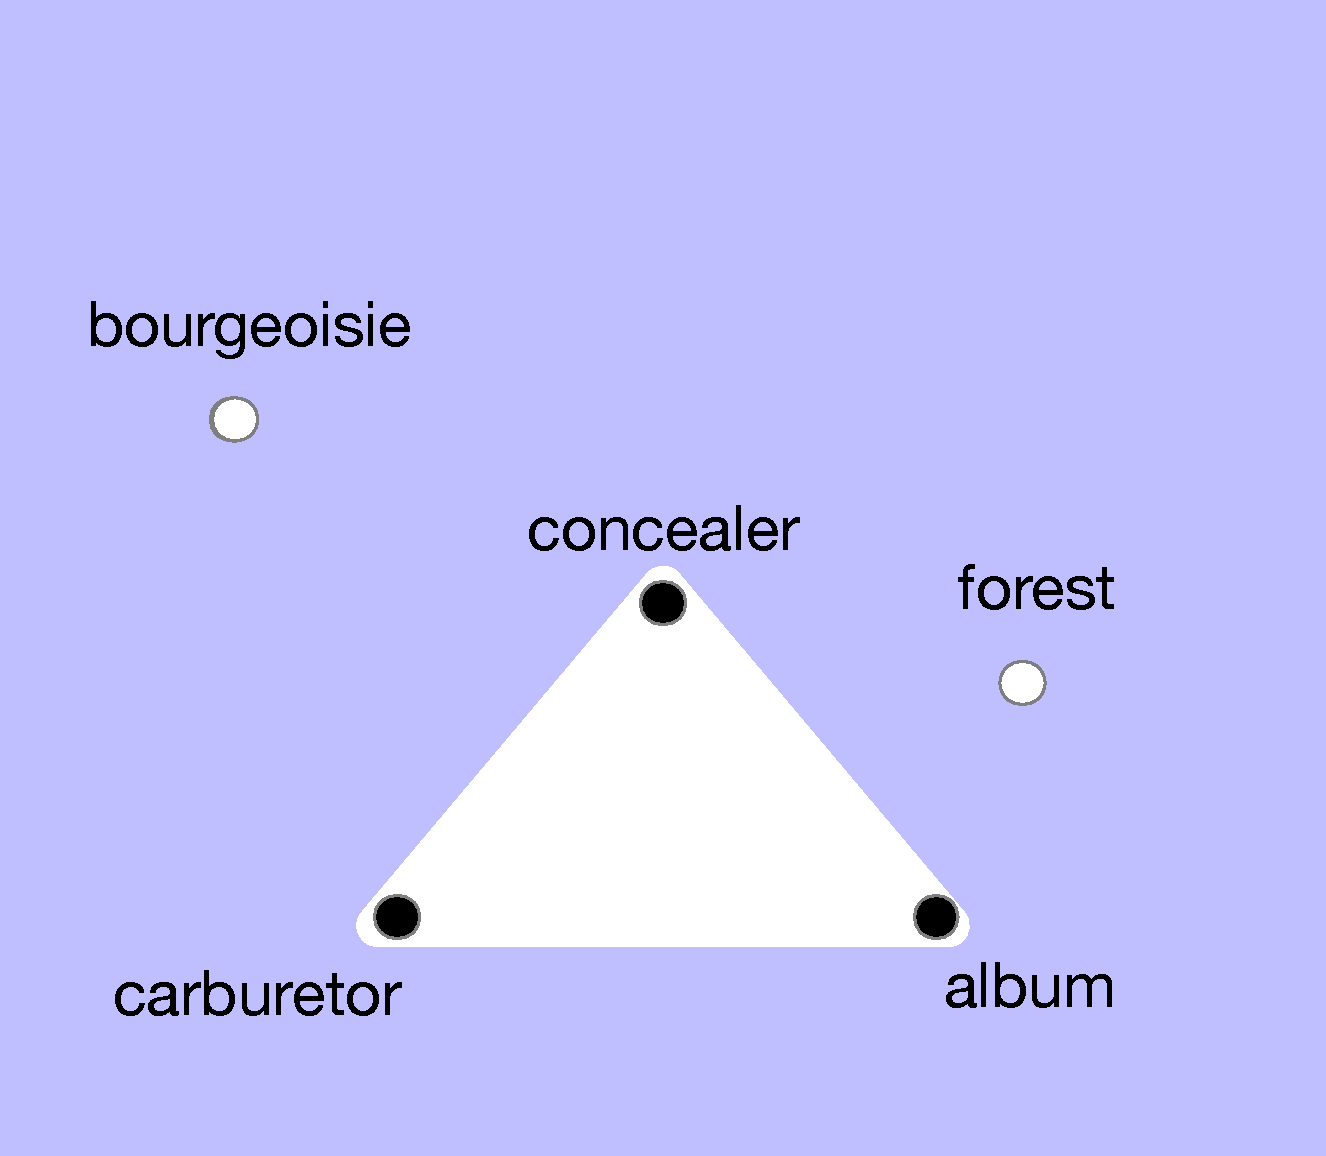
\includegraphics[width=0.8\linewidth]{mono_anchors1}
    \end{figure}

	\vspace{3cm}
    
    To greedily find an anchor word, find a row in $\bar{Q}$ that is farthest away from the current span of anchor words.
    \begin{figure}
	\centering
	
	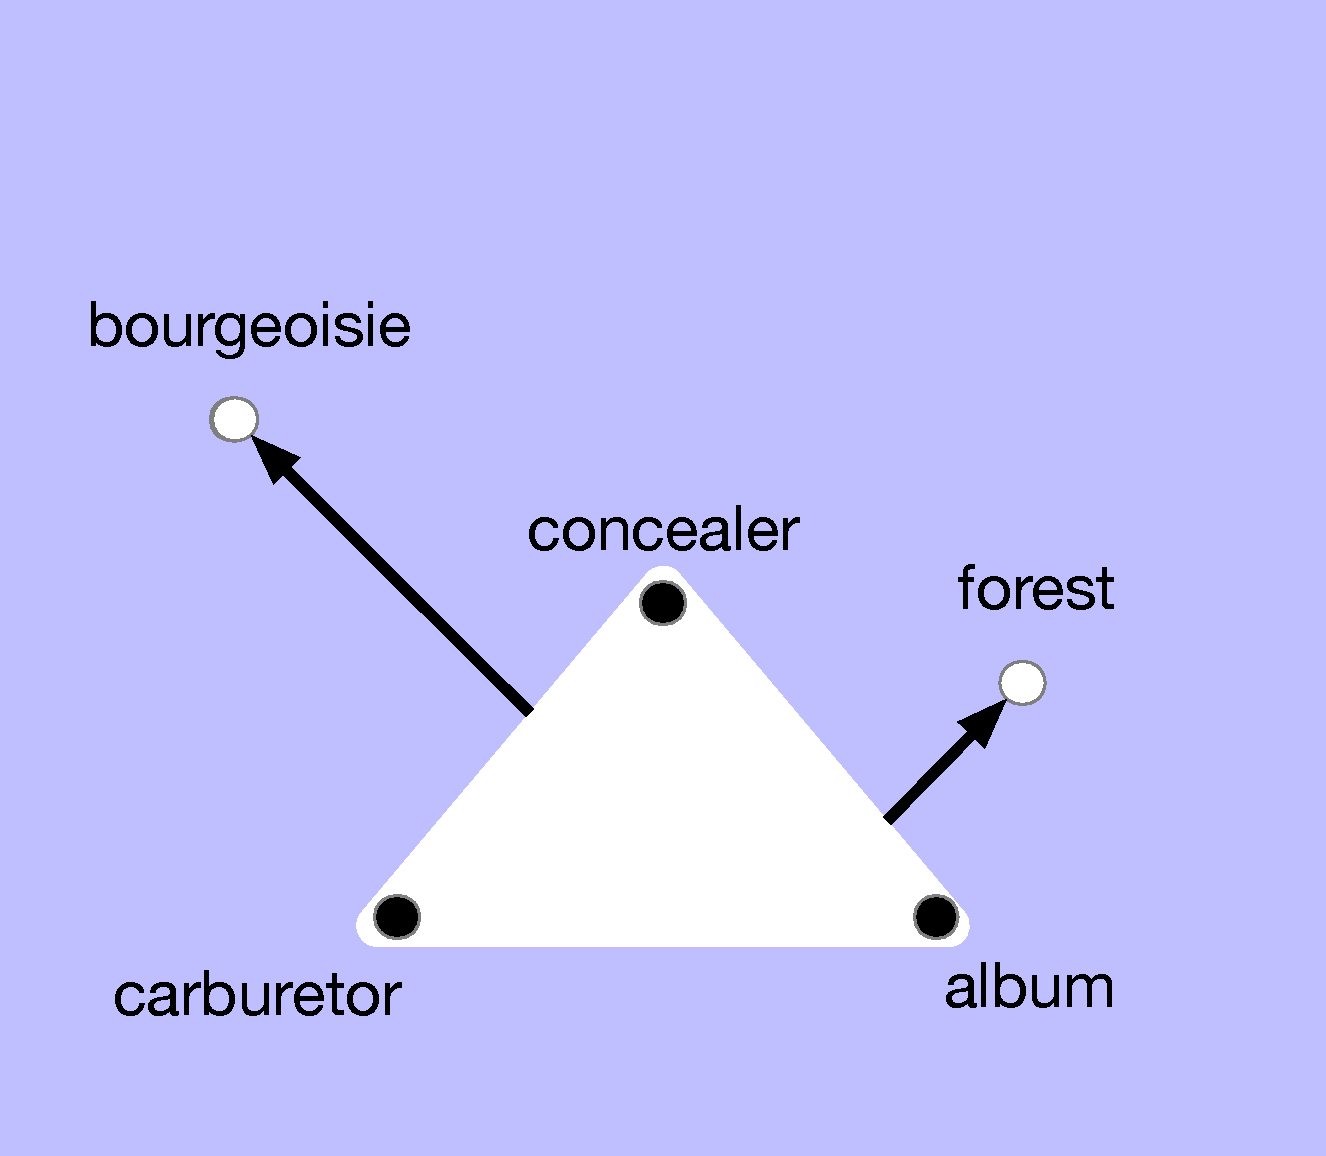
\includegraphics[width=0.8\linewidth]{mono_anchors2}
\end{figure}

\vspace{3cm}

The goal is to maximize total span of anchor words so that each row in $\bar{Q}$ lies within this span and can be accurately approximated. 

    \begin{figure}
	\centering
	
	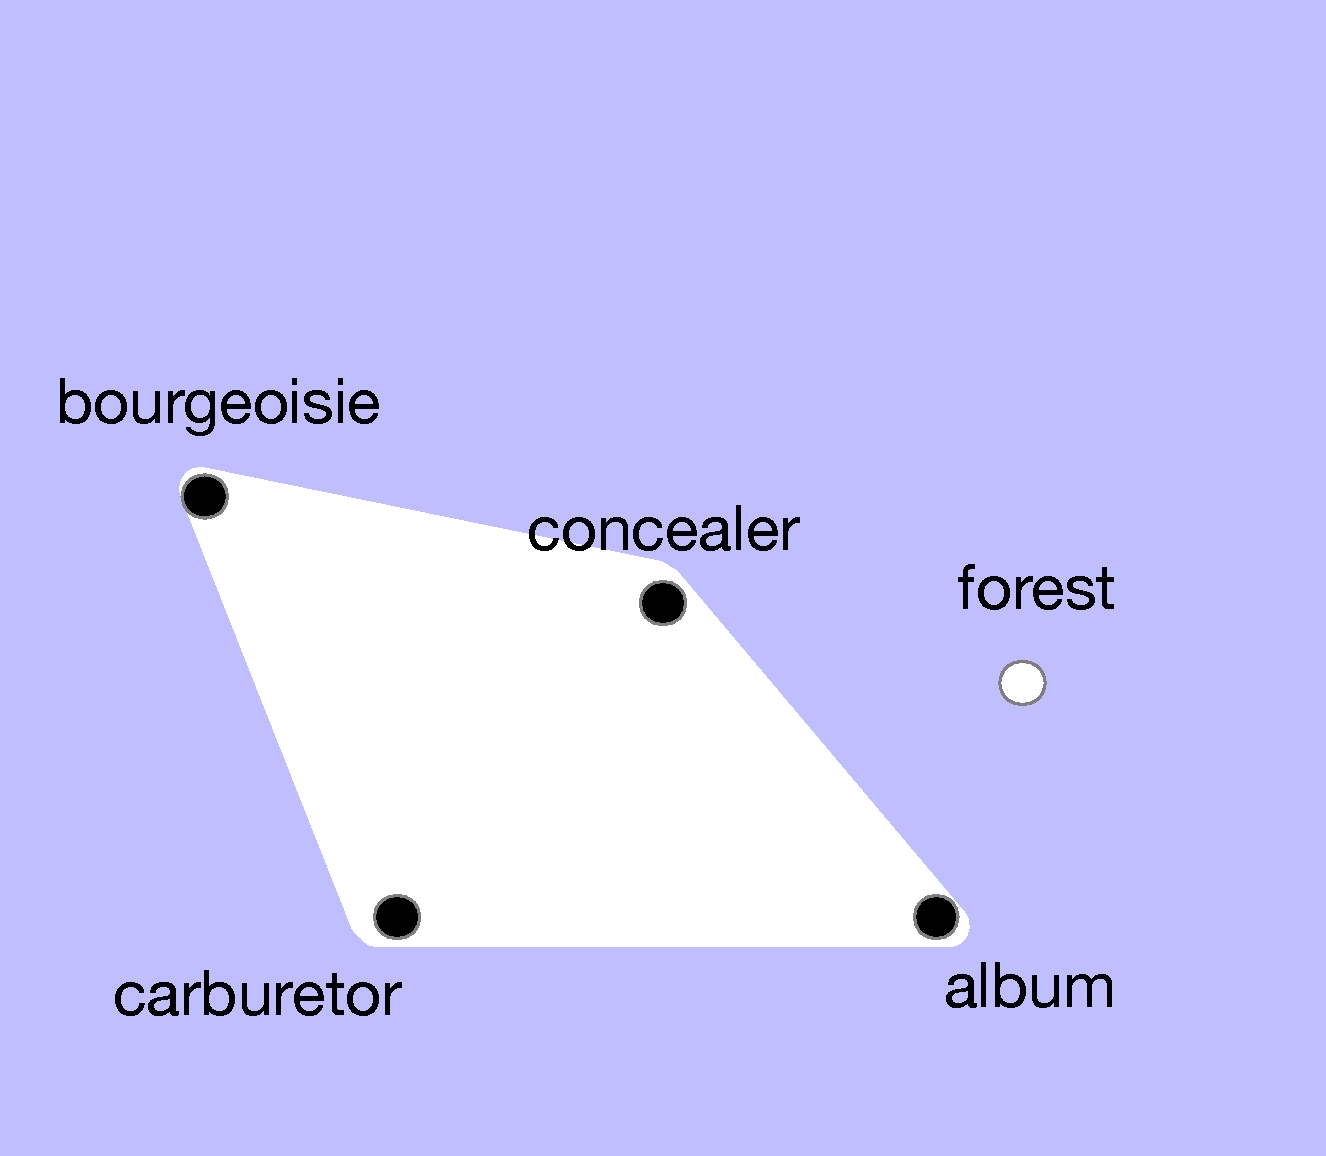
\includegraphics[width=0.8\linewidth]{mono_anchors3}
\end{figure}

    
\end{column}

\begin{column}{0.67\textwidth}
\header{Multilingual Anchoring}

The challenge for multilingual topic modeling is to align topics cross-lingually even when words from different languages do not co-occur in the same documents.

   \begin{figure}
	\centering
	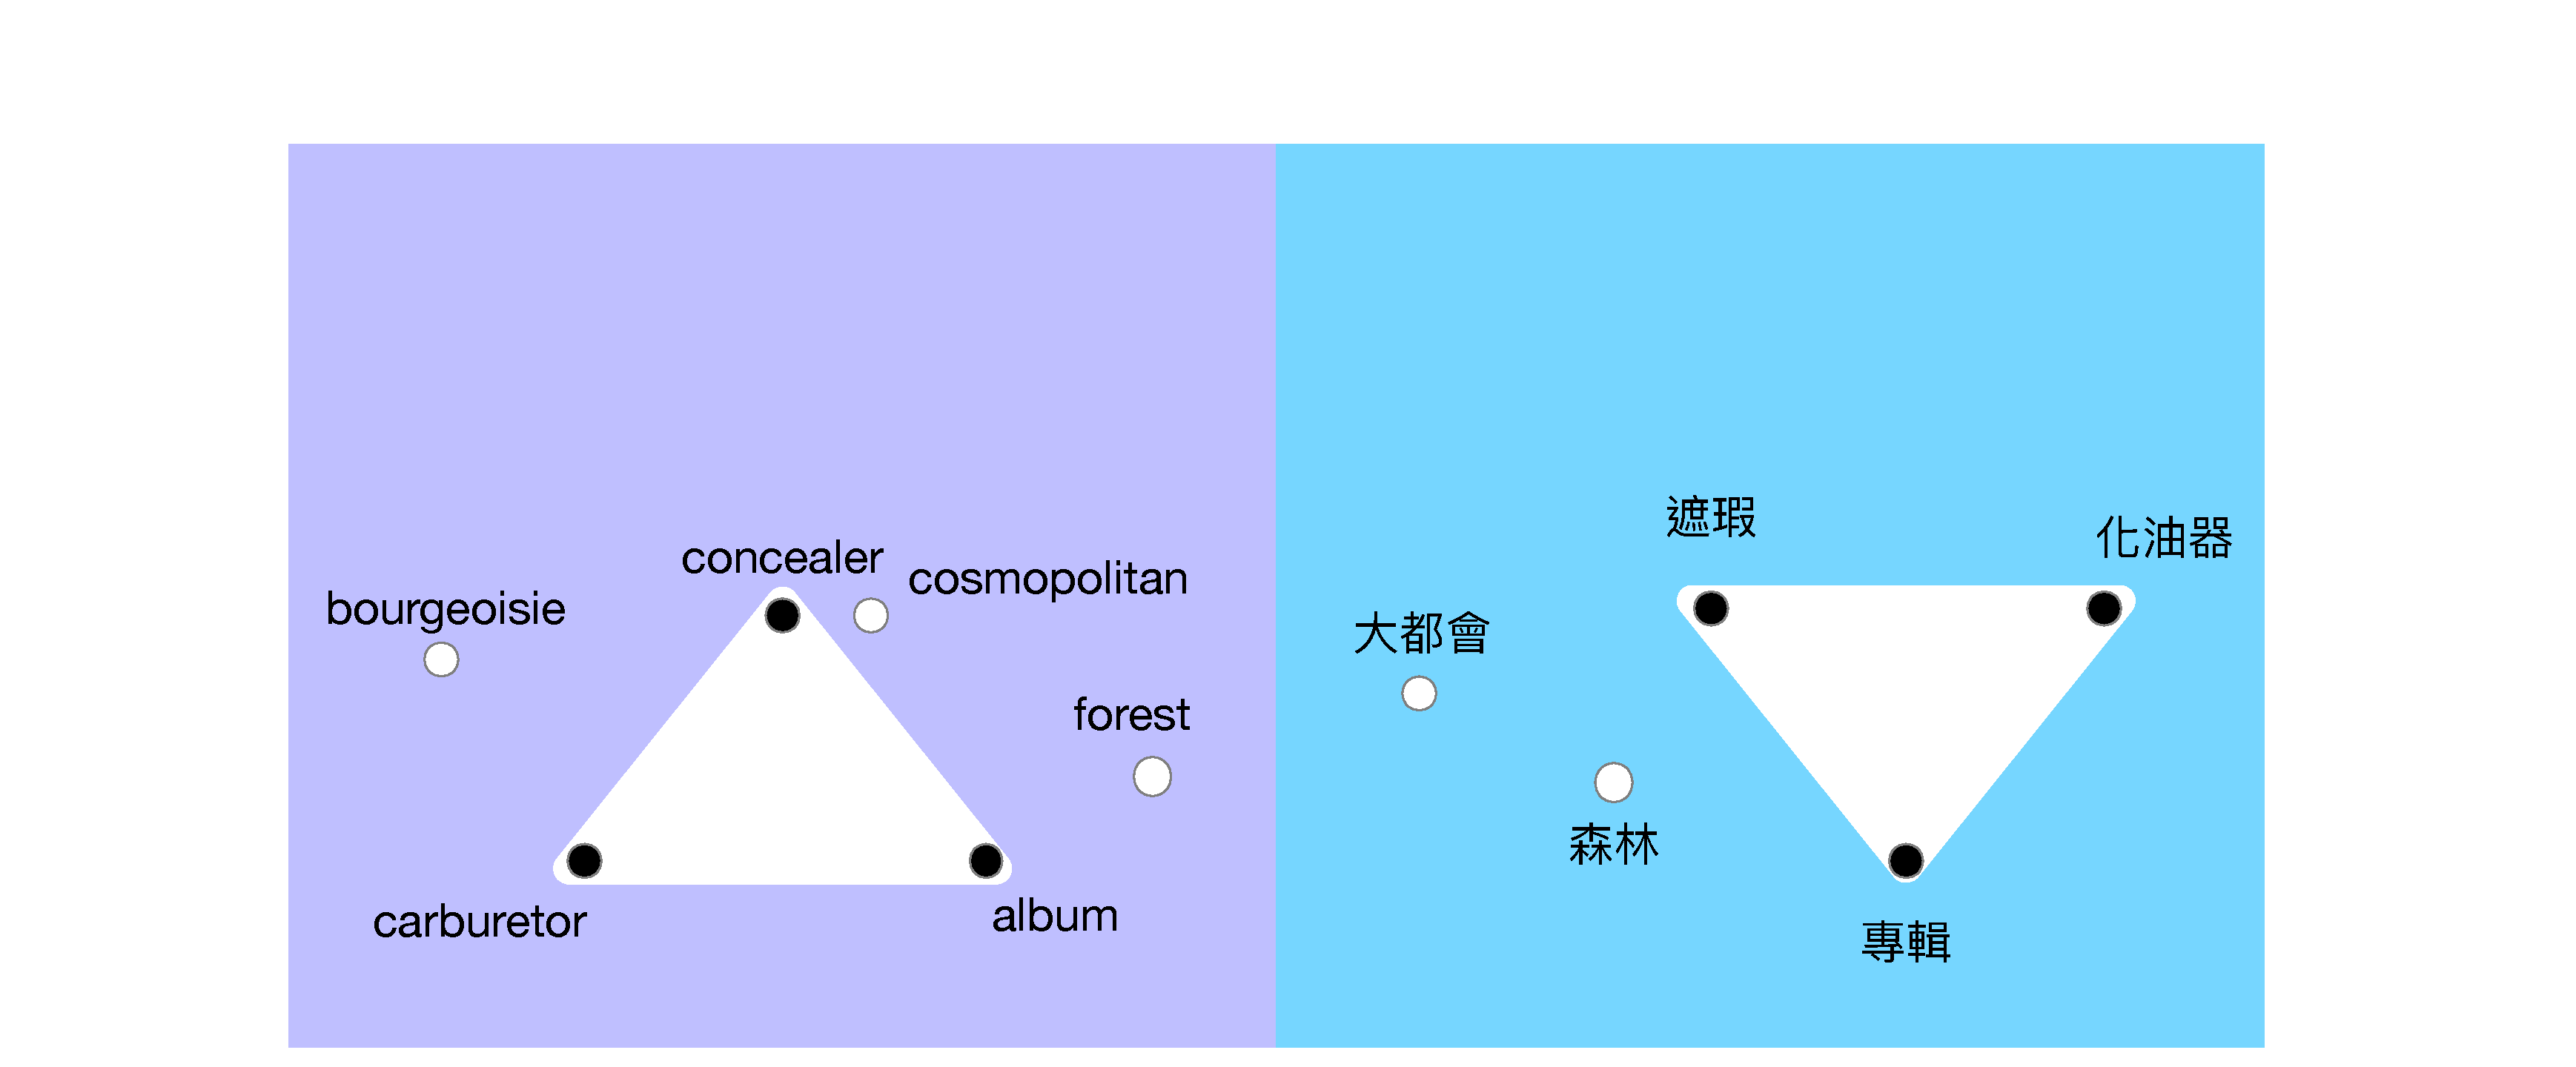
\includegraphics[width=\linewidth]{multi_anchors1}
\end{figure}

\vspace{5cm}

Our algorithm first uses a dictionary to link words across languages.

\begin{figure}
	\centering
	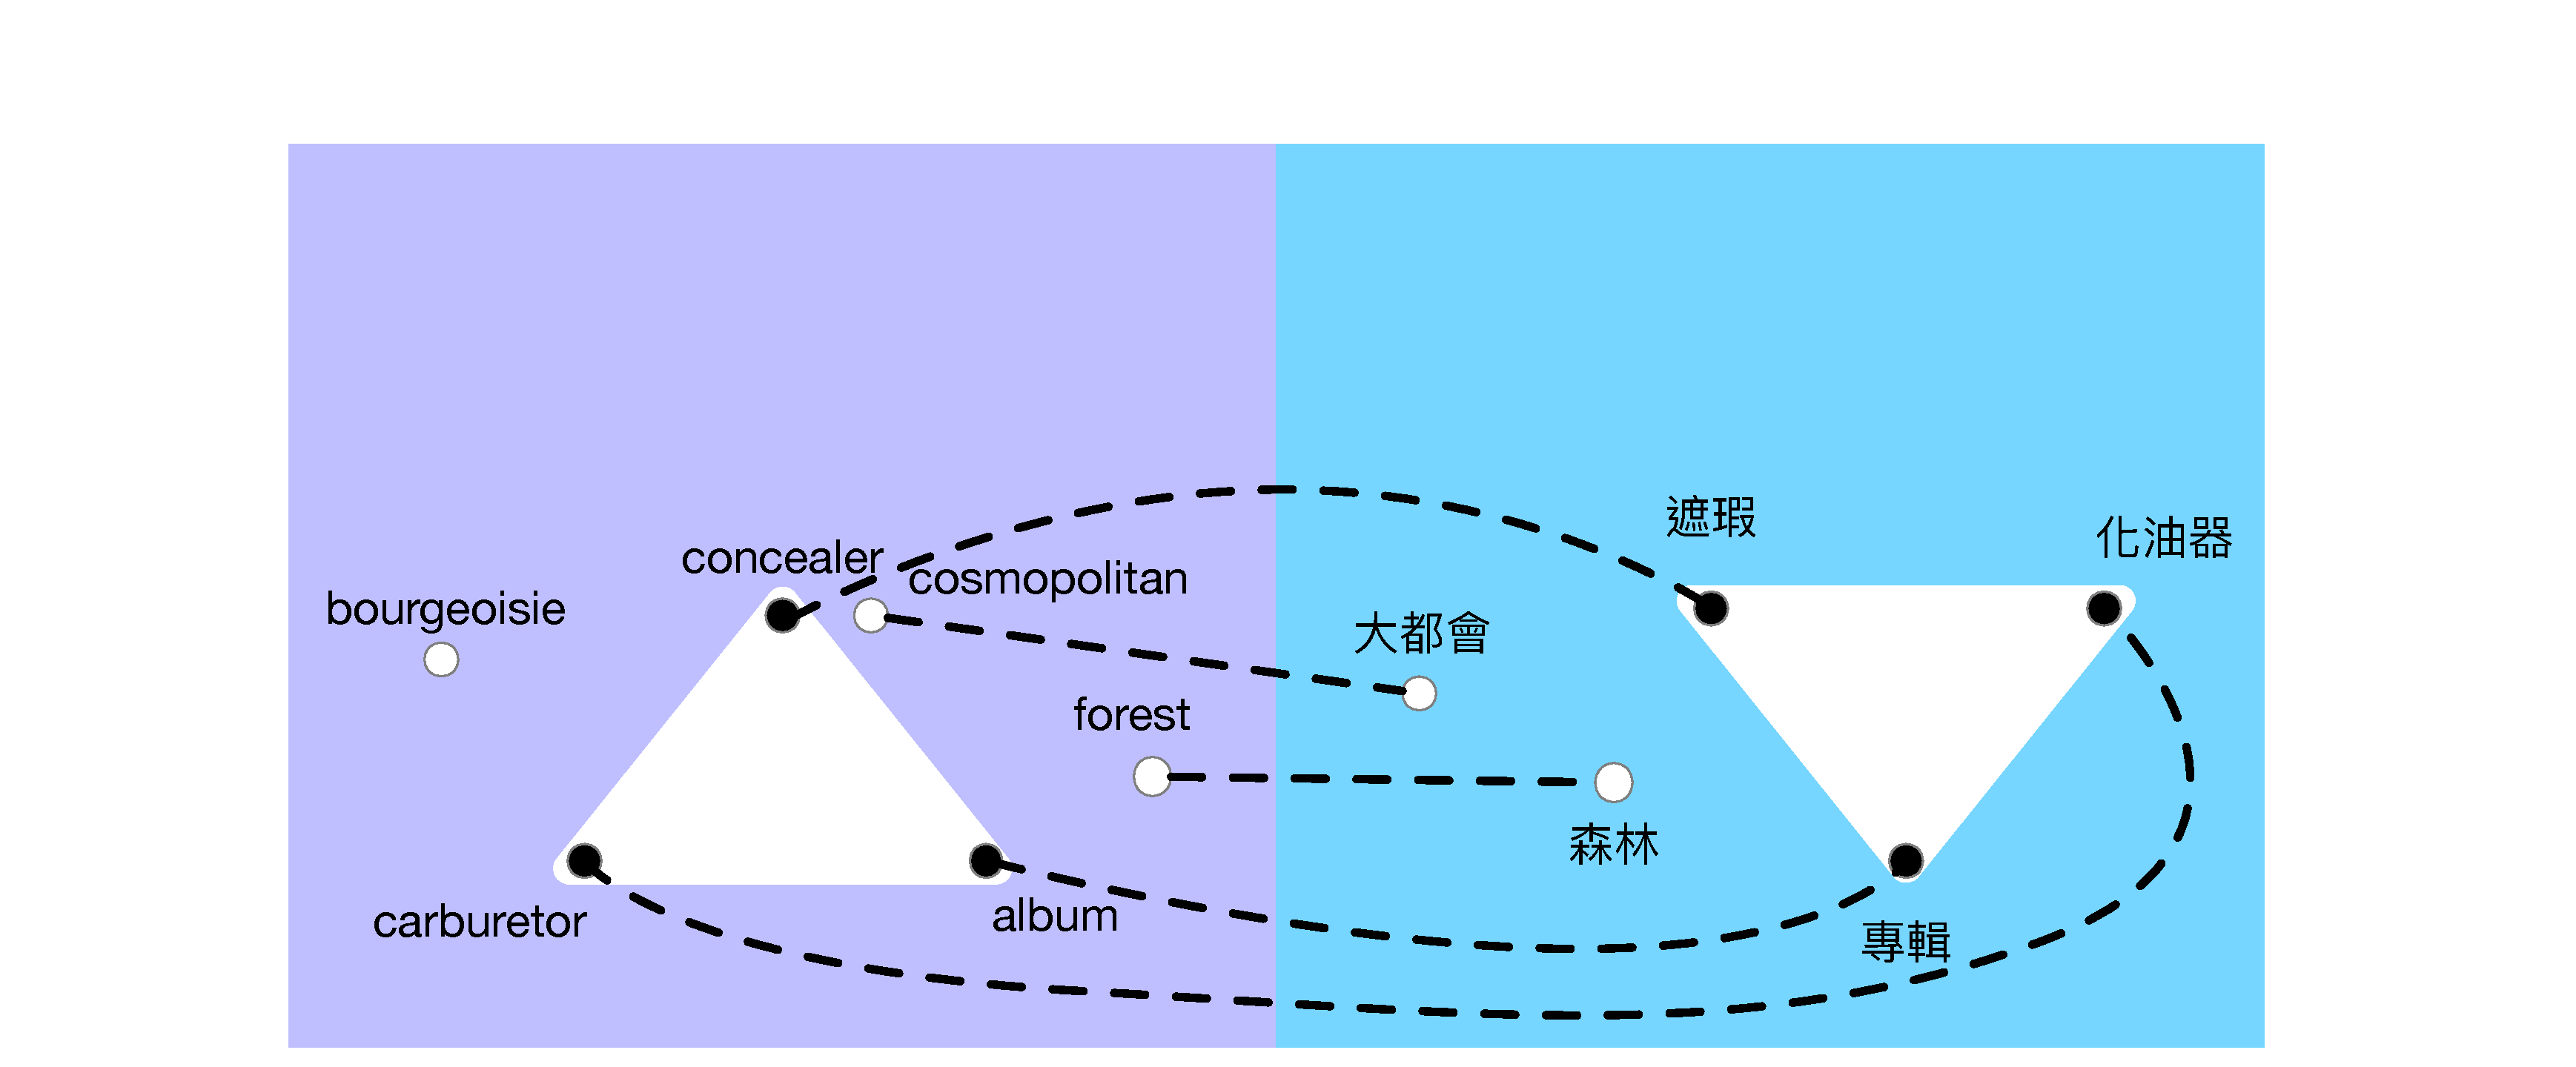
\includegraphics[width=\linewidth]{multi_anchors2}
\end{figure}

\vspace{5cm}

Then, it finds anchor words such that they are linked and can simultaneously expand the span of anchors words for both languages.

\begin{figure}
	\centering
	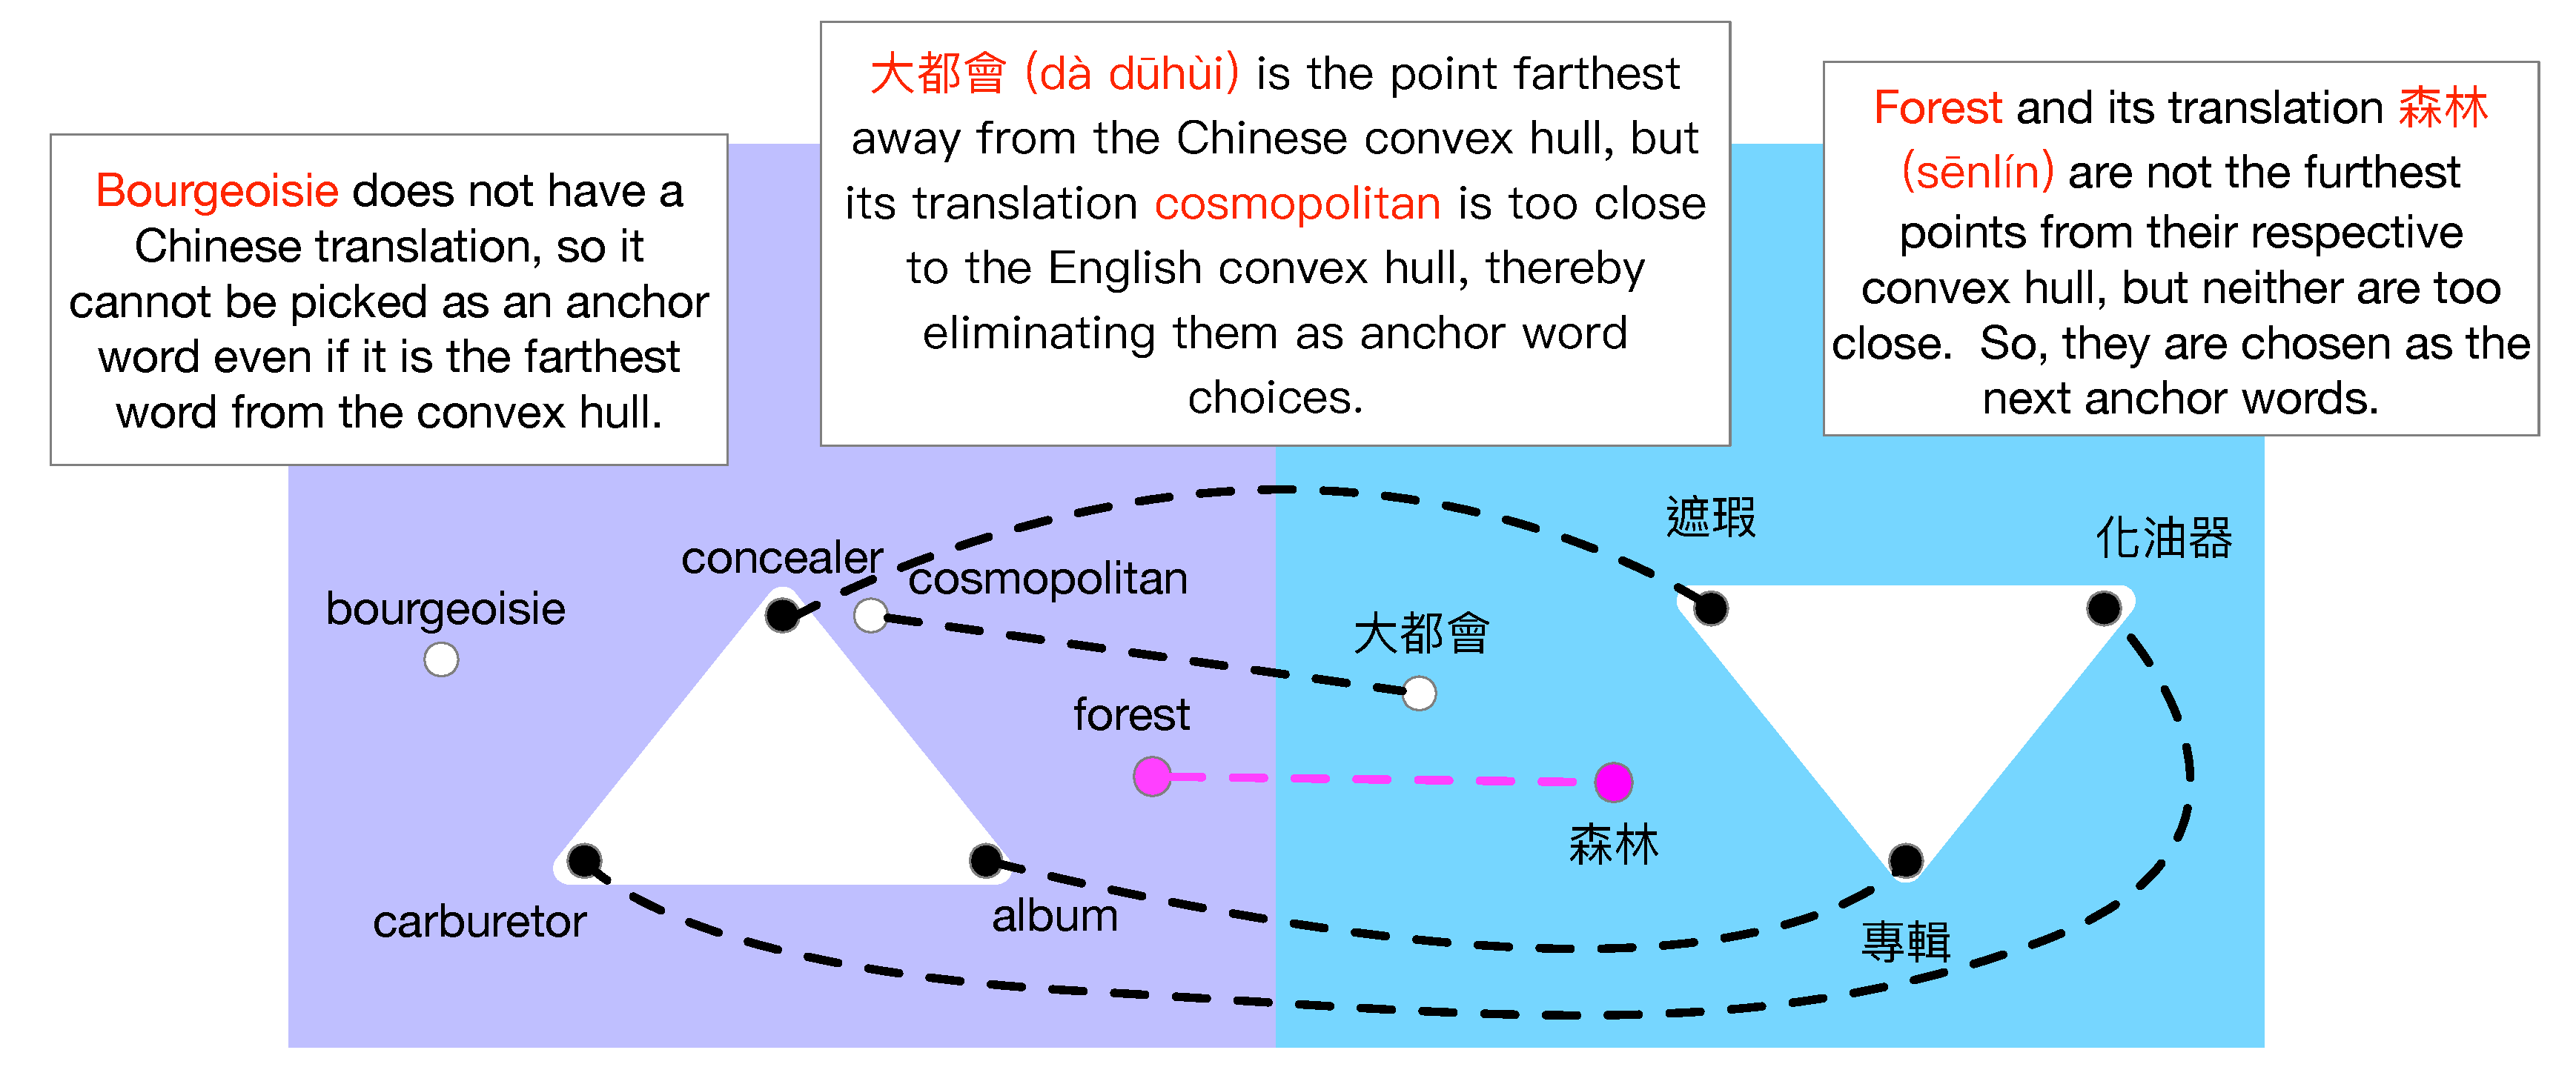
\includegraphics[width=\linewidth]{multi_anchors6}
\end{figure}

\end{column}
\end{columns}

\end{block}


\end{column}

\separatorcolumn


\begin{column}{\colwidth}
	
	\begin{block}{MTAnchor: Interactive Topic Modeling}
		
		\header{User Interface}
		\begin{figure}
			\centering
			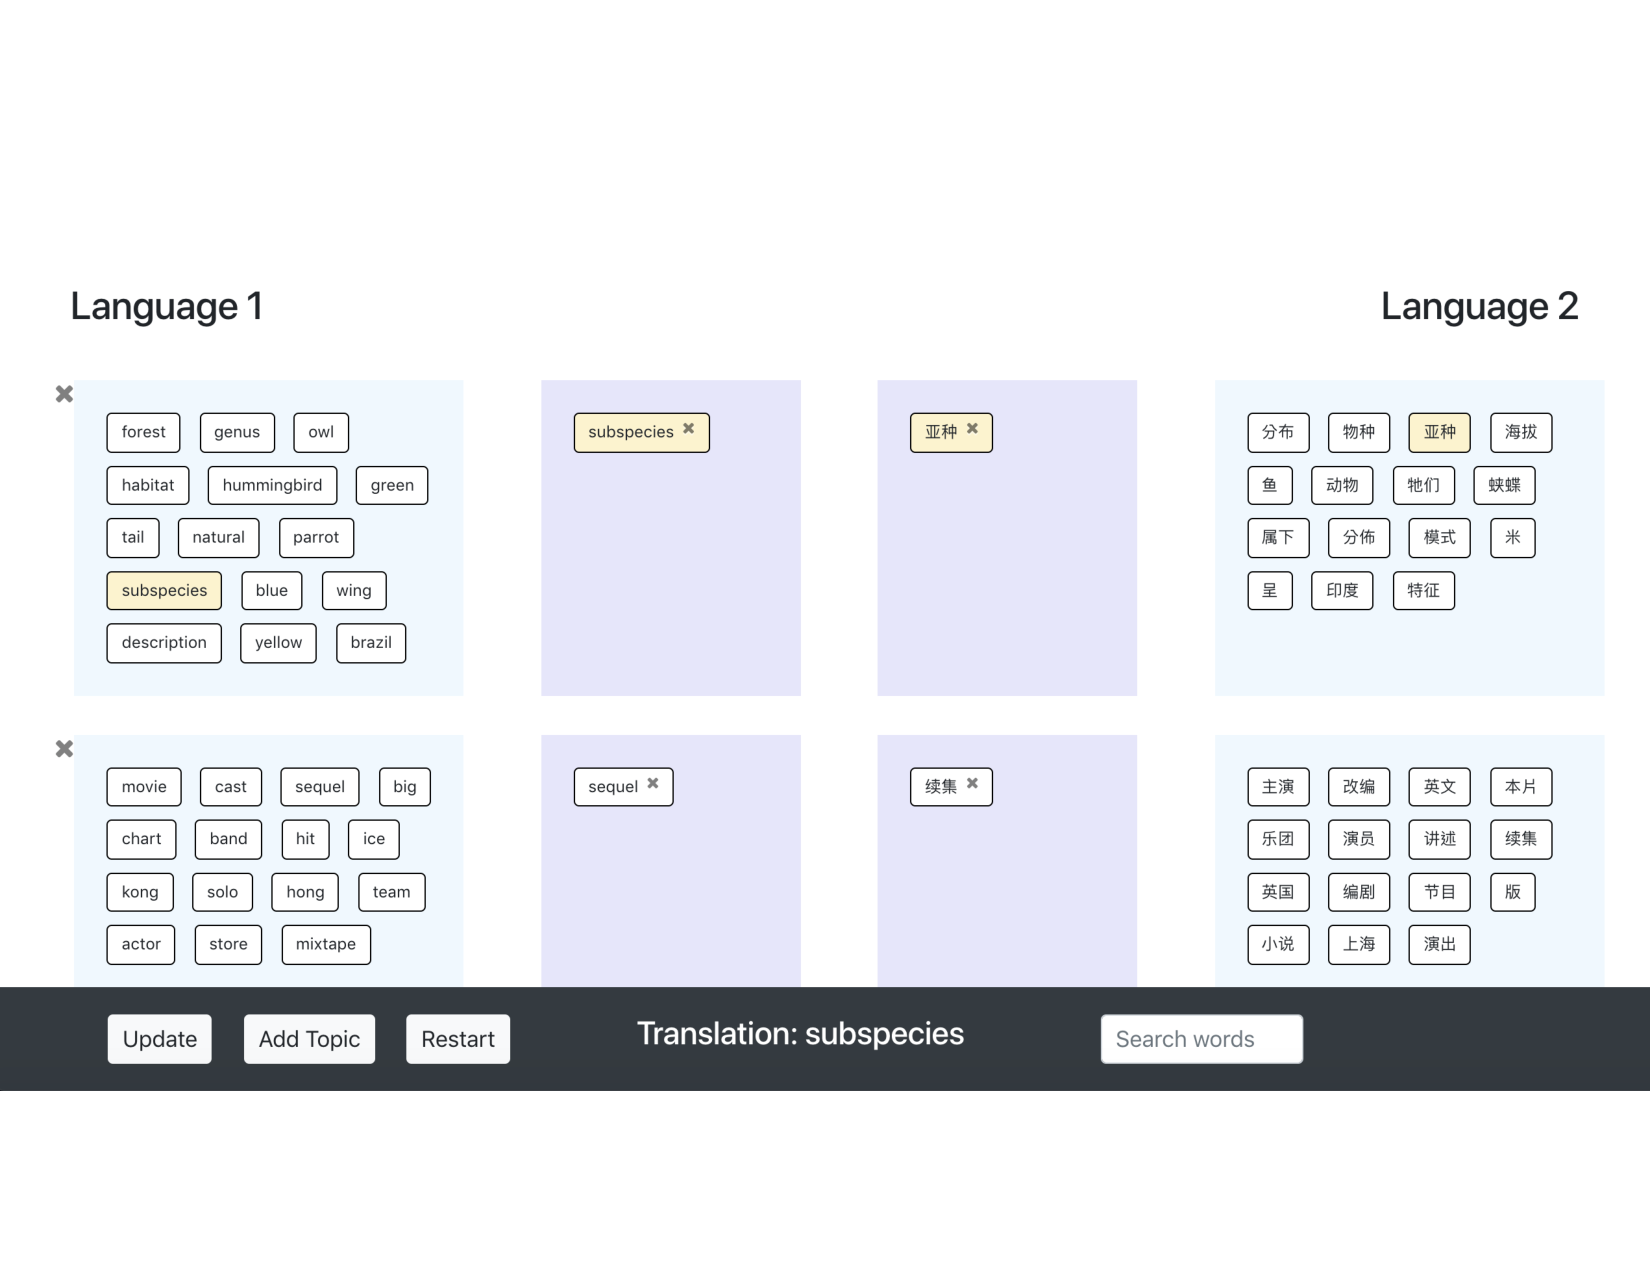
\includegraphics[width=0.8\linewidth]{ui_final}
		\end{figure}
	
		\vspace{2cm}
			
		\header{User Study}
%		We invited twenty users through Mechanical Turk to participate in the user study.  Each participant was given a maximum of thirty minutes to interact with MTAnchor.  The graphs below show the changes in classification accuracy (using topics as features) over time.
		\begin{figure}
			\centering
			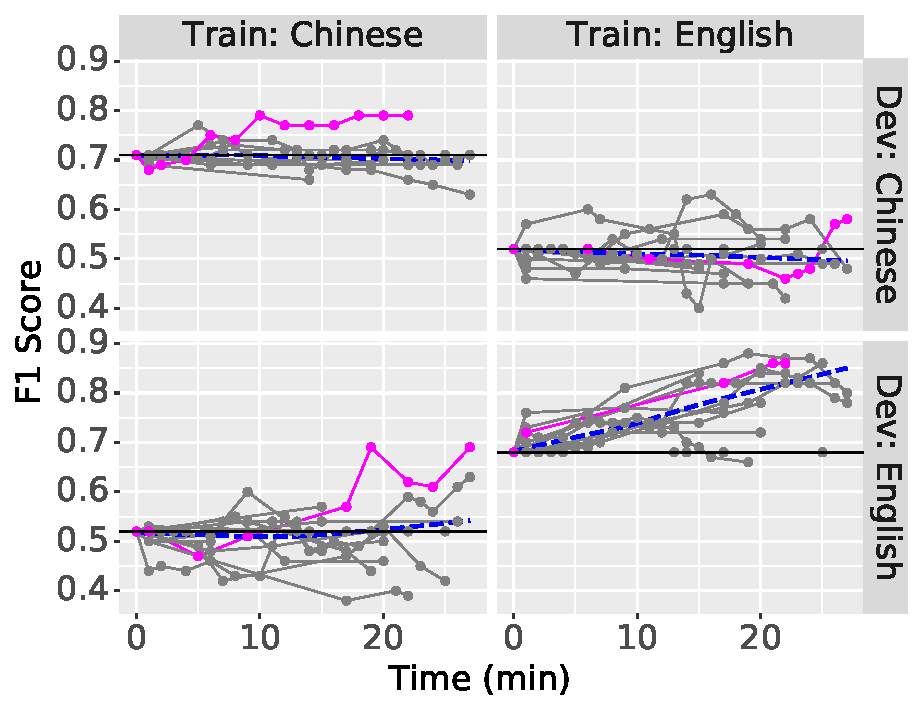
\includegraphics[width=0.6\linewidth]{user_exp} 
		\end{figure}
		\begin{figure}
			\centering
			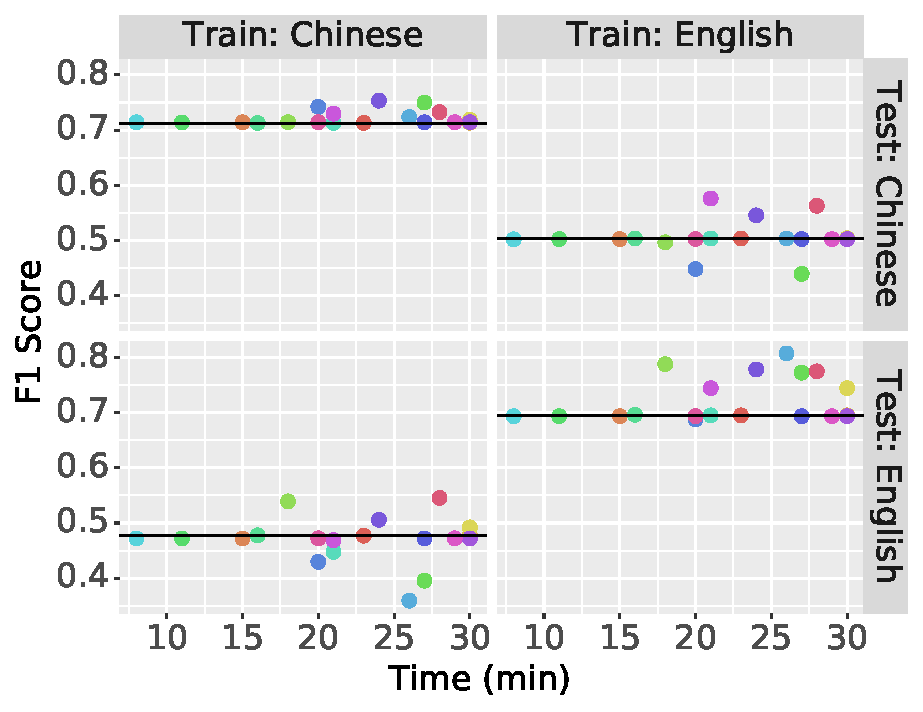
\includegraphics[width=0.6\linewidth]{usertest}
		\end{figure}
		
	\end{block}
	
	\vspace{2cm}
	  \begin{alertblock}{More Information}
	
	\begin{itemize}
	\item Code: \url{https://github.com/forest-snow/mtanchor_demo/}
	\item Author: 
	\url{http://www.cs.umd.edu/~myuan/}
	\item This work was supported in part by the JHU Human Language Technology Center of Excellence (HLTCOE) and Raytheon BBN Technologies, by DARPA award HR0011-15-C-0113.
	\end{itemize}
	
	  \end{alertblock}
  
\end{column}

\separatorcolumn

\begin{column}{0.75\colwidth}

  \begin{block}{Comparing Models}
  	
\header{Speed and Classification Accuracy}
    \begin{figure}
    	\centering
    	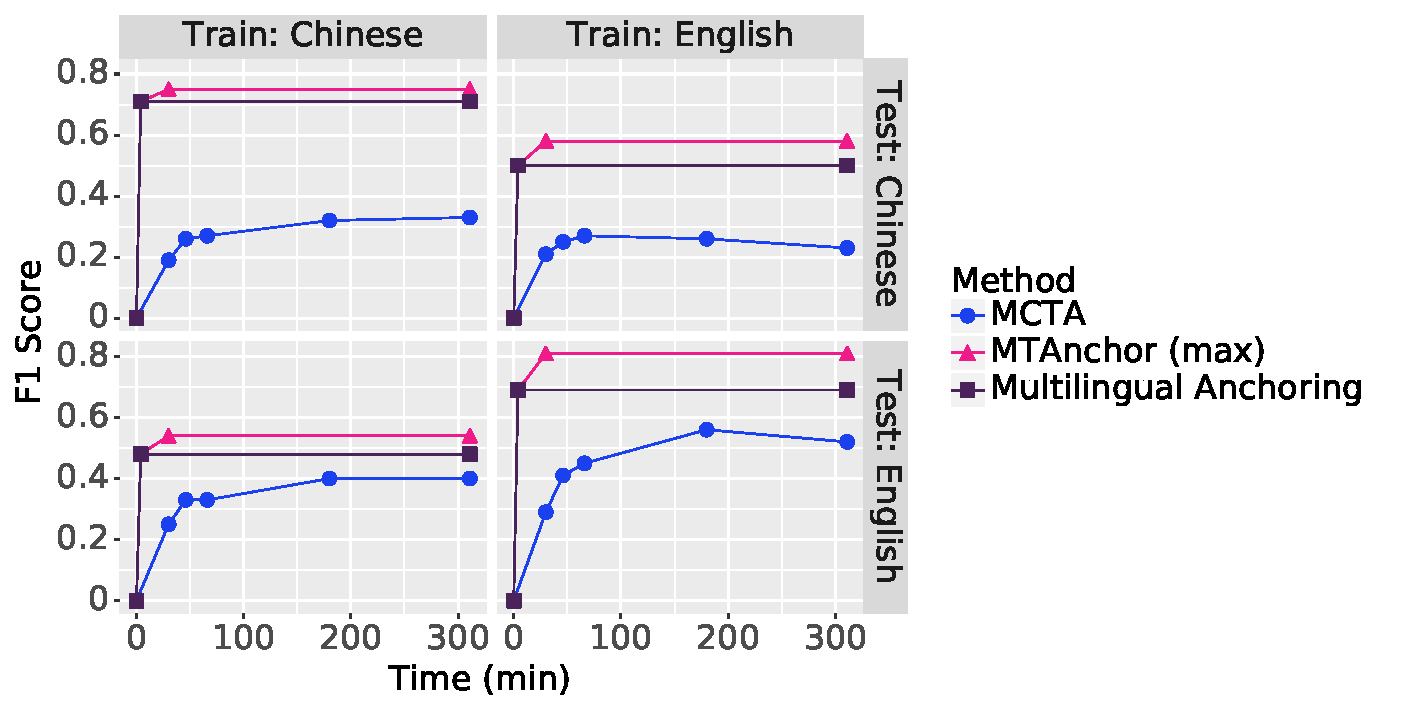
\includegraphics[width=0.8\linewidth]{methods_wiki}
    \end{figure}

	
\header{Topic Coherence}
\begin{table}
	\centering
	\scriptsize
	\begin{tabular}{llllll} \\
		& & \multicolumn{4}{c}{Topic coherence} \\
		\cmidrule(r){3-6}
		Dataset & Method & \abr{en-i} & \makecell{\abr{zh-i}\\\abr{si-i}} & \abr{en-e} & \makecell{\abr{zh-e}\\\abr{si-e}} \\
		\midrule 
		Wikipedia & \makecell{Multilingual\\anchoring} & 0.14 & 0.18 & 0.08 & 0.13  \\
		& \makecell{\mtanchor\\(maximum)} & \textbf{0.20} & \textbf{0.20} & \textbf{0.10} & \textbf{0.15} \\
		& \makecell{\mtanchor\\(median)} & 0.14 & 0.18 & 0.08 & 0.13\\
		& \abr{mcta} & 0.13 & 0.09 & 0.00 & 0.04  \\
		\midrule
		Amazon & \makecell{Multilingual\\anchoring} & \textbf{0.07} & \textbf{0.06} & \textbf{0.03} & \textbf{0.05} \\
		& \abr{mcta} & -0.03 & 0.02 & 0.02 & 0.01 \\
		\midrule 
		\abr{lorelei} & \makecell{Multilingual\\anchoring} & 0.08 & 0.00 & 0.03 & n/a \\
		& \abr{mcta} & \textbf{0.13} & 0.00 & \textbf{0.04} & n/a  \\
	\end{tabular}
\end{table}



\header{Sample Film Topic}
\begin{figure}
	\centering
	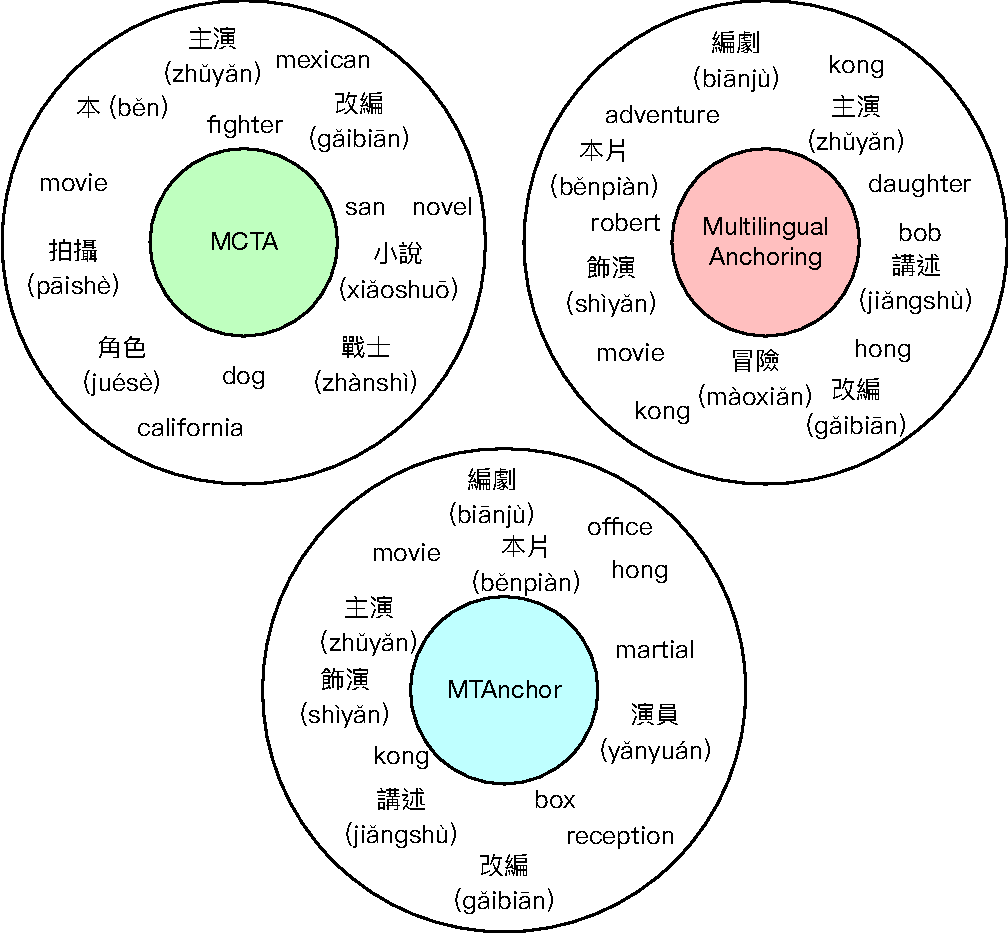
\includegraphics[width=0.8\linewidth]{topics}
\end{figure}

  \end{block}

\begin{block}{Conclusions}
	\begin{itemize}
		\item Anchoring algorithm can be applied multilingually
		\item People can provide helpful linguistic and cultural knowledge to improve topic models
	\end{itemize}
\end{block}



\end{column}

\edgecolumn




\end{columns}
\end{frame}

\end{document}
